\documentclass[12pt]{article}
\usepackage[letterpaper, margin=1in]{geometry}
\usepackage[acronym]{glossaries}
\usepackage[automake]{glossaries-extra}
\usepackage{graphicx}
\usepackage{float}

% Document font setup %
\usepackage{charter}

% TITLE PAGE INFORMATION %
\title{Carleton University InSpace On-Board Telemetry System Design}
\author{Matteo Golin}
\date{
    November 19, 2023 \\
    Modified: \today
}

% GLOSSARY %
% ACRONYMS %
\newacronym{pr}{PR}{Pull Request}
\newacronym{ui}{UI}{User Interface}
\newacronym{cuinspace}{CUInSpace}{Carleton University InSpace}
\newacronym{rtos}{RTOS}{Real-Time Operating System}
\newacronym{lora}{LoRa}{Long Range}
\newacronym{srad}{SRAD}{Student Researched And Designed}
\newacronym{cots}{COTS}{Commercial Off-The-Shelf}
\newacronym{posix}{POSIX}{Portable Operating System Interfaced based on UNIX}
\newacronym{ipc}{IPC}{Inter-Process Communication}
\newacronym{i2c}{I2C}{Inter-Integrated Circuit}
\newacronym{uart}{UART}{Universal Asynchronous Receiver/Transmitter}
\newacronym{html}{HTML}{Hyper Text Markup Language}

% GLOSSARY DEFINITIONS %
\newglossaryentry{qnx}{
    name=QNX,
    description={Blackberry's microkernel real-time operating system}
}
\newglossaryentry{unix}{
    name=Unix,
    description={An operating system invented at Bell Labs which inspired a family of operating systems and POSIX
            standards}
}
\newglossaryentry{posixgls}{
    name=POSIX,
    description={A set of standards by the IEEE which define compatible operating system interfaces}
}
\newglossaryentry{stdin}{
    name=stdin,
    description={The standard input stream used by POSIX compliant operating systems, which takes console input}
}
\newglossaryentry{stderr}{
    name=stderr,
    description={The standard error stream used by POSIX compliant operating systems, which outputs errors to the console}
}
\newglossaryentry{stdout}{
    name=stdout,
    description={The standard output stream used by POSIX compliant operating systems, which outputs data to the console}
}
\newglossaryentry{fifo}{
    name=FIFO,
    description={First-In-First-Out; a file-like buffer implemented by POSIX systems}
}
\newglossaryentry{gnu}{
    name=GNU,
    description={GNU's Not Unix; a collection of free software which can be used standalone or as an operating system}
}
\newglossaryentry{agile}{
    name=agile,
    description={A software development methodology characterized by short bursts of development efforts with a focus on
            continuously delivering a functioning product. This methodology does not make use of heavy testing or a
            sequential development life-cycle, but rather tackles challenges as they appear}
}
\newglossaryentry{standup}{
    name=standup,
    description={A short meeting which takes place every day of a sprint in the Agile development methodology. This
            meeting usually lasts no longer than 10 minutes, giving developers an opportunity to quickly recount the status of
            their current tasks}
}
\newglossaryentry{vmodel}{
    name=V-model,
    description={A software development methodology inspired by the Waterfall method, with a focus on associating each step of
            the development cycle with testing requirements}
}
\newglossaryentry{githubpages}{
    name=GitHub pages,
    description={A static web-page hosting service provided by GitHub, allowing web pages in a GitHub repository to be
            made visible via a public URL}
}

\makeglossaries

% MAIN DOCUMENT %
\begin{document}

% TITLE %
\maketitle
\pagebreak

% TABLE OF CONTENTS %
\tableofcontents
\pagebreak

% OVERVIEW %
\section{Overview}

This document covers the design of the \glsxtrfull{cuinspace} on-board telemetry system. The telemetry system uses
\gls{qnx}'s \glsxtrfull{rtos} and modular processes in order to achieve the goal of transmitting sensor data collected
from an \glsxtrfull{srad} sensor board over \glsxtrfull{lora} radio to \glsxtrshort{cuinspace}'s \glsxtrshort{srad}
ground station.

\subsection{Context}

The \glsxtrshort{cuinspace} telemetry system design must maintain compatibility with the existing ground station
software and telemetry packet format specification. It must use \glsxtrshort{lora} radio to communicate telemetry
packets to be consistent with previous designs.

The telemetry system must also be able to read sensor data from \glsxtrshort{srad} sensor boards of different designs
using \glsxtrfull{i2c}. It must complete all these responsibilities while being as conservative as possible in power
usage so as to preserve enough battery life for flight while idling on the launch pad.

Another important consideration of this system is maintainability. The system must be well documented, easily
extensible and maintainable. It must be approachable for new \glsxtrshort{cuinspace} members so that developers are
able to complete new features and tasks in a reasonable amount of time regardless of initial software development
knowledge or progress in their undergraduate degree.


% TECHNICAL ARCHITECTURE %
\section{Technical Architecture}

The \glsxtrshort{cuinspace} telemetry system software will be composed of multiple modules:

\begin{enumerate}
    \setlength{\itemsep}{1pt}
    \setlength{\parskip}{0pt} \setlength{\parsep}{0pt}
    \item \texttt{controller}
    \item \texttt{fetcher}
    \item \texttt{packager}
    \item \texttt{broadcaster}
    \item \texttt{writer}
\end{enumerate}

\subsection{Architecture Diagrams}

The architecture for the \glsxtrshort{cuinspace} telemetry system is separated into two system designs:
\begin{enumerate}
    \setlength{\itemsep}{1pt}
    \setlength{\parskip}{0pt} \setlength{\parsep}{0pt}
    \item Critical functionality for the 2023-2024 telemetry system (Figure \ref{fig:crit-arc})
    \item Non-critical functionality which can be postponed to 2024-2025 (Figure \ref{fig:non-crit-arc})
\end{enumerate}

\begin{figure}[H]
    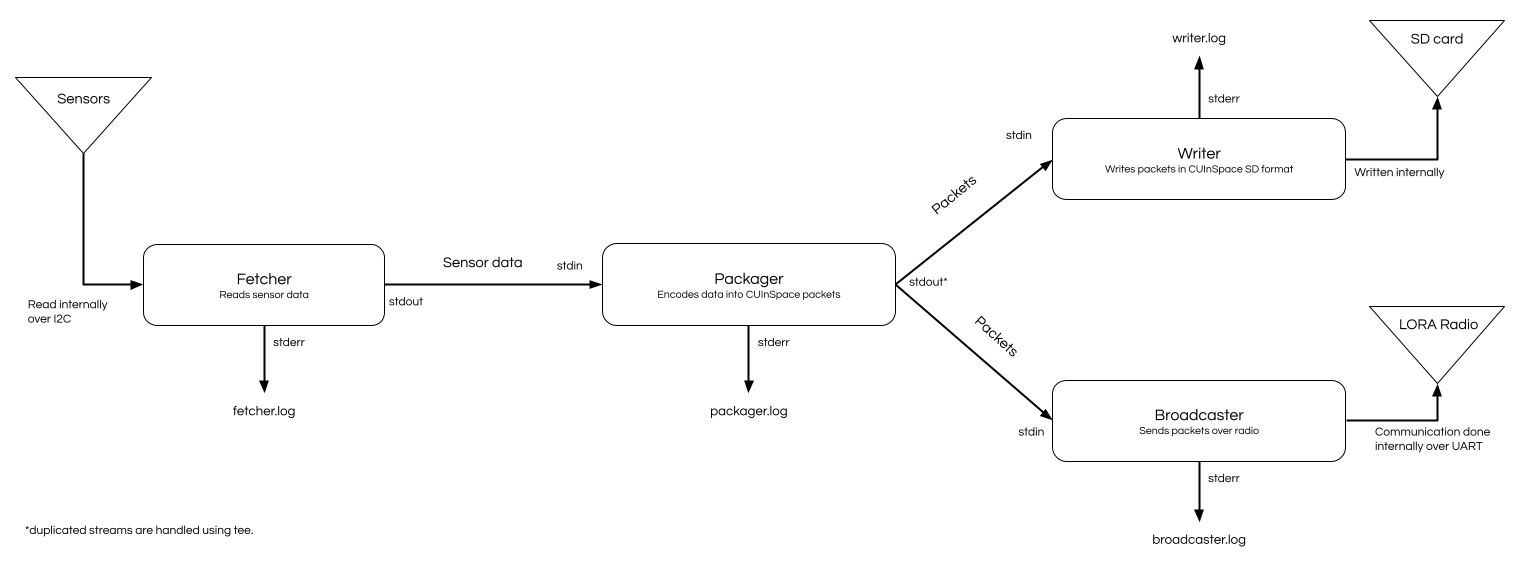
\includegraphics[width=\linewidth]{assets/critical-architecture.png}
    \caption{System diagram of the critical functionality for the telemetry system}
    \label{fig:crit-arc}
\end{figure}

\begin{figure}[H]
    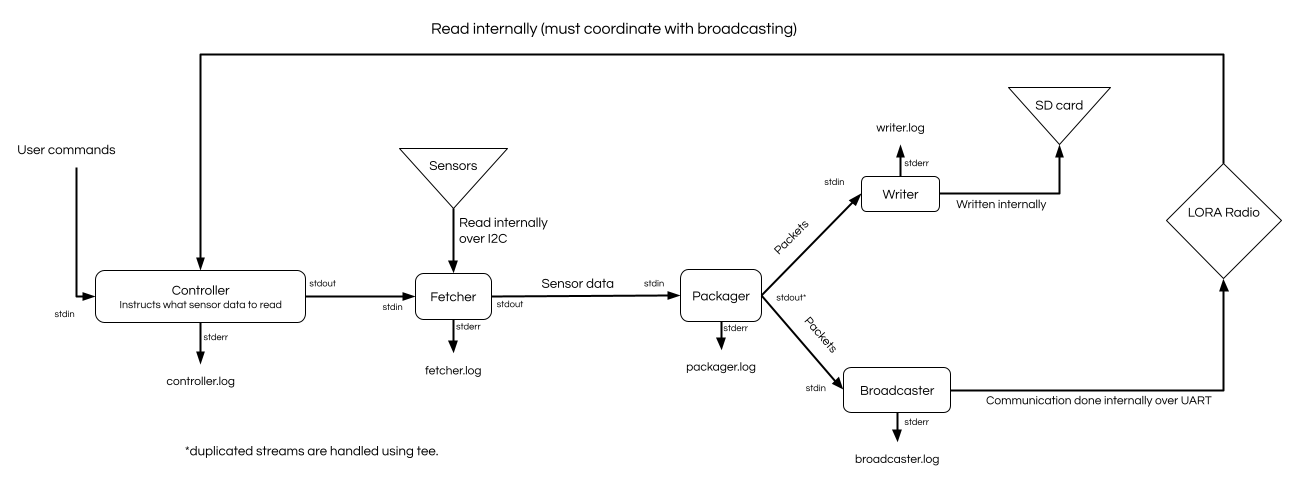
\includegraphics[width=\linewidth]{assets/non-critical-architecture.png}
    \caption{System diagram of the non-critical functionality for the telemetry system}
    \label{fig:non-crit-arc}
\end{figure}

\subsection{Modules} \label{s:modules}

Each module makes use of the \gls{unix} philosophy: do one task, and do it well. Modules are \glsxtrfull{posix}
compliant in order to be portable across other \glsxtrshort{posix} compliant \glsxtrshortpl{rtos}. As part of the
adoption of the \gls{unix} philosophy, each module will also expect their input in plain-text (where applicable) and
provide their output in plain text. This allows each module's output to be useful on its own as well as part of the
whole system, rather than being tailored for input into another module. Additionally, a plain-text output makes it
easier for developers to reason about and debug module output.

All of the modules are written in the C programming language, in order to make use of \gls{qnx}'s included C libraries.
This also facilitates \glsxtrshort{srad} development, as members in the engineering and computer science programs
become familiar with C programming early in their undergraduate degree.

All modules use \texttt{\gls{stdin}}, \texttt{\gls{stdout}} and \texttt{\gls{stderr}} for \glsxtrfull{ipc}. Error
messages and logs are sent to \texttt{\gls{stderr}} so that they can be easily separated from other program output and
redirected to a log file. Modules read their input from \texttt{\gls{stdin}} to be processed, and write their output to
\texttt{\gls{stdout}}. This allows for modules to be piped into each other easily. Modules will also be able to read
from a file or a \gls{fifo} in addition to \texttt{\gls{stdin}} for more control using output duplication with the
\gls{posixgls} \texttt{tee} command.

None of the libraries developed for use in the modules make assumptions about memory allocation, and instead accept
pre-allocated memory blocks to initialize with data. This allows modules to be portable to embedded systems with less
development overhead.

All modules are bundled with help text which can be displayed with the \texttt{use} command. The help text contains a
description of the module, its usage, example calls, and command line options and their default values.

All modules follow the gnu11 C standard. This standard was selected because it is a modern C standard which permits the
use of \gls{gnu} libraries (such as \texttt{getopt}, a library for \glsxtrshort{posix} compliant command line
interfaces).

\subsubsection{Controller}

\textbf{This module is not part of the critical functionality for the 2023-2024 \glsxtrshort{cuinspace} telemetry
    system.}

The \texttt{controller} module is responsible for receiving control commands from the ground station over
\glsxtrshort{lora} and providing them to \texttt{fetcher} for interpretation. The \glsxtrshort{cuinspace} packet format
specification (\ref{a:telem-format}) describes control packets which allow the ground station to request only specific
types of telemetry data from the rocket telemetry system. The \texttt{controller} module will read these control
packets from the \glsxtrshort{lora} RN2483 chip and provide them as plain-text instructions to the \texttt{fetcher}
module.

The \texttt{controller} module will also be able to provide signal reports and check the \glsxtrshort{lora} radio
settings. It may later be required to take input from an interactive terminal interface so that the telemetry system
can be monitored by developers. The module will also have the ability to modify radio parameters in accordance with the
control packets it receives from the ground station.

\subsubsection{Fetcher}

The \texttt{fetcher} module is responsible for perpetually reading sensor data. It does so by reading data from all the
sensors on the \glsxtrshort{cuinspace} \glsxtrshort{srad} sensor board via an \glsxtrshort{i2c} bus.

The \texttt{fetcher} module will output sensor data in plain-text, human readable measurements via
\texttt{\gls{stdout}}. Outputted sensor data will be annotated with its data type (altitude, temperature, etc.) and
unit of measurement.

The \texttt{fetcher} module will be able to receive instructions about which sensor data to prioritize via
\texttt{\gls{stdin}}. It will also be able to accept a configuration which specifies sensor addresses, sensor data
types (altitude, temperature, etc.) and commands for reading from the sensors in order to be configurable for different
\glsxtrshort{srad} sensor boards. \textbf{This functionality is not part of the critical requirements for the 2023-2024
    telemetry system}.

\subsubsection{Packager}

The \texttt{packager} module is responsible for packaging sensor data into the \glsxtrshort{cuinspace} telemetry packet
format. It requires an HAM radio call sign provided via command line in order to sign all the packets that it creates.
\texttt{packager} will write the encoded radio packets to \texttt{\gls{stdout}} in plain-text hexadecimal digits.

\subsubsection{Broadcaster}

The \texttt{broadcaster} module is responsible for interfacing with the \glsxtrshort{lora} RN2483 radio chip over
\glsxtrshort{uart} to broadcast messages to the ground station. It accepts input in the form of plain-text hexadecimal
digits over \texttt{\gls{stdin}} (or a file), which it sends to the radio chip for transmission. Newline characters in
the input signify the end of a transmission. \texttt{broadcaster} will also accept command line options for all of the
configurable radio parameters provided by the RN2483 radio chip, which it will use for transmission.

\subsubsection{Writer}

The \texttt{writer} module is responsible for writing \glsxtrshort{cuinspace} telemetry packets to an SD card using the
\glsxtrshort{cuinspace} SD card storage format.

\subsection{Build System}

The build system for all software modules will be implemented using \gls{make}. \Gls{make} was chosen because of its
simplicity and wide adoption across software projects, especially C projects. The command line utility is available for
Windows and \glsxtrshort{posix} operating systems, and a version of it is included with the \gls{qnx} build system for
consistency across machines.

The \gls{make} build system also integrates with \gls{qnx}'s existing build system to recursively compile and link the
provided libraries. \Gls{qnx}'s build system also allows automatic building of multiple executables for different
architectures with the addition of sub directories to the project directory. \cite{qnx-dir-structure} The build system
can also bundle executables with their help documentation for integration with the \texttt{use} command.
\cite{qnx-dir-structure}


% GLOSSARY %
\pagebreak
\printglossary[type=\acronymtype,title=Acronyms]
\printglossary[title=Glossary]

\end{document}
